\chapter{Exploring $N = 2$ with a Leapfrog Algorithm}

During their next session, Alice, Bob, and Carol wrote a second-order
integrator, with Bob behind the key board this time.  They chose the
leapfrog algorithm, one of the most popular integrators for cases
where only modest accuracy is needed.  In some cases the problem
itself does not require high accuracy.  In other cases the leapfrog is
used to quickly build a prototype, a toy model that can give insight
in the overall structure of the problem.  At a later stage, once the
overall strategy has become more clear, a higher-order integrator can
replace the leapfrog.  Dense stellar systems are an example of the
latter category, where fourth-order algorithms are almost always the
engines of choice in $N$-body codes.

We will not follow their dialogue in detail here, but rather describe
a summary of their results.

\section{Two Ways to Write the Leapfrog}

The name {\it leapfrog} comes from one of the ways to write this
algorithm, where positions and velocities `leap over' each other.
Positions are defined at times $t_i, t_{i+1}, t_{i+2}, \dots $, spaced
at constant intervals $dt$, while the velocities are defined at times
halfway in between, indicated by $t_{i-1/2}, t_{i+1/2}, t_{i+3/2}, \dots $,
where $t_{i+1} - t_{i + 1/2} = t_{i + 1/2} - t_i = dt / 2$.  
The leapfrog integration scheme then reads:

\begin{eqnarray}
\br_{i} & = & \br_{i-1} + \bv_{i-1/2} dt \label{leapfrog-leap-step1} \\
\bv_{i+1/2} & = & \bv_{i-1/2} + \ba_i dt \label{leapfrog-leap-step2}
\end{eqnarray}

Note that the accelerations $\ba$ are defined only on integer times,
just like the positions, while the velocities are defined only on
half-integer times.  This makes sense, given that $\ba(\br, \bv) = \ba(\br)$:
the acceleration on one particle depends only on its position with respect
to all other particles, and not on its or their velocities.  Only at
the beginning of the integration do we have to set up the velocity at
its first half-integer time step.  Starting with initial conditions
$\br_0$ and  $\bv_0$, we take the first term in the Taylor series
expansion to compute the first leap value for $\bv$:

\begin{equation}
\bv_{1/2} = \bv_0 + \ba_0 dt / 2.
\end{equation}

We are then ready to apply Eq. \ref{leapfrog-leap-step1} to compute
the new position $\br_1$, using the first leap value for $\bv_{1/2}$.
Next we compute the acceleration $\ba_1$, which enables us to compute
the second leap value, $\bv_{3/2}$, using Eq. \ref{leapfrog-leap-step2},
and so on.

A second way to write the leapfrog looks quite different at first sight.
Defining all quantities only at integer times, we can write:

\begin{eqnarray}
\br_{i+1} & = & \br_i + \bv_{i} dt + \ba_{i} (dt)^2/2 \label{leapfrog-step1} \\
\bv_{i+1} & = & \bv_i + (\ba_i + \ba_{i+1})dt / 2 \label{leapfrog-step2}
\end{eqnarray}

This is still the same leapfrog scheme, although represented in a
different way.  Notice that the increment in $\br$ is given by the
time step multiplied by $\bv_{i}  + \ba_{i} dt/ 2$, effectively equal
to $\bv_{i+ 1/2}$.  Similarly, the increment in $\bv$ is given by the
time step multiplied by $(\ba_i + \ba_{i+1}) / 2$, effectively equal
to the intermediate value $\ba_{i+1/2}$.  In conclusion, although both
positions and velocities are defined at integer times, their
increments are governed by quantities approximately defined at
half-integer values of time.

A most interesting way to see the equivalence of
Eqs. \ref{leapfrog-leap-step1}, \ref{leapfrog-leap-step2} and 
Eqs. \ref{leapfrog-step1}, \ref{leapfrog-step2} is to note the fact
that the first two equations are explicitly time-reversible, while it
is not at all obvious whether the last two equations are time-reversible.
For the two systems to be equivalent, they'd better share this property.
Let us inspect.

Starting with Eqs. \ref{leapfrog-leap-step1}, \ref{leapfrog-leap-step2},
even though it may be obvious, let us write out the time reversibility.
We will take one step forward, taking a time step $+dt$, to evolve
$\{\br_i, \bv_{i-1/2}\}$ to $\{\br_{i+1}, \bv_{i+1/2}\}$, and then we
will take one step backwards, using the same scheme, taking a time
step $-dt$.  Clearly, the time will return to the same value since
$+dt-dt=0$, but we have to inspect where the final positions and
velocities $\{\br_f(t=i), \bv_f(t=i-1/2)\}$ are indeed equal to their
initial values $\{\br_i, \bv_{i-1/2}\}$.  Here is the calculation, resulting
from applying Eqs. \ref{leapfrog-leap-step1}, \ref{leapfrog-leap-step2} twice.

\begin{eqnarray}
\br_f & = & \br_{i+1} - \bv_{i+1/2} dt \nonumber \\
      & = & \left[ \br_i + \bv_{i+1/2} dt \right]
            - \bv_{i+1/2} dt \nonumber \\
      & = & \br_i \\
                  \nonumber \\
\bv_f & = & \bv_{i+1/2} - \br_i dt \nonumber \\
      & = & \left[ \bv_{i-1/2} + \ba_i dt \right]
            - \ba_i dt \nonumber \\
      & = & \bv_{i-1/2}
\end{eqnarray}

In an almost trivial way, we can see clearly that time reversal causes
both positions and velocities to return to their old values, not only
in an approximate way, but exactly.  In a computer application, this
means that we can evolve forward a thousand time steps and then evolve
backward for the same length of time.  Although we will make
integration errors (remember, leapfrog is only second-order, and thus
not very precise), those errors will exactly cancel each other, apart
from possible round-off effects, due to limited machine accuracy.

Now the real fun comes in, when we inspect the equal-time
Eqs. \ref{leapfrog-step1}, \ref{leapfrog-step2}:

\begin{eqnarray}
\br_f & = & \br_{i+1} - \bv_{i+1} dt + \ba_{i+1} (dt)^2/2 \nonumber \\
      & = & \left[ \br_i + \bv_i dt + \ba_i (dt)^2/2 \right]
            - \left[ \bv_i + (\ba_i + \ba_{i+1})dt / 2 \right] dt
            + \ba_{i+1} (dt)^2/2 \nonumber \\
      & = & \br_i \\
                  \nonumber \\
\bv_f & = & \bv_{i+1} - (\ba_{i+1} + \ba_i)dt / 2  \nonumber \\
      & = & \left[ \bv_i + (\ba_i + \ba_{i+1})dt / 2 \right]
            - (\ba_{i+1} + \ba_i)dt / 2  \nonumber \\
      & = & \bv_i
\end{eqnarray}

In this case, too, we have exact time reversibility.  Even though not
immediately obvious from an inspection of Eqs. \ref{leapfrog-step1},
\ref{leapfrog-step2}, as soon as we write out the effects of stepping
forward and backward, the cancellations become manifest.

\section{A Simple Leapfrog for the 2-Body Problem}

Our friends decided to write their leapfrog scheme using the second
way of implementing the algorithm, centering all physical quantities
on integer time step times.

The first leapfrog code that Bob wrote, {\st leapfrog1.C}, is similar
to the last forward Euler code that they produced, at the end of the
previous chapter, {\st forward\_euler3.C}.  There are really only two
differences.  One is a computation of the acceleration before we get
into the integration loop, and the other is the difference in the
integration steps themselves.  Here is the code:

\code{leapfrog1.C}{chap4/leapfrog1.C}

Let us start with the integration loop {\st for (double t = 0; \dots}.
A direction implementation of Eqs. \ref{leapfrog-step1}, \ref{leapfrog-step2}
would have give for the third and fourth line of the loop:

\begin{small}
\begin{verbatim}
            r[k] += v[k] * dt + 0.5 * a[k] * dt * dt;
            v[k] += 0.5 * a[k] * dt;
\end{verbatim}
\end{small}

\noindent
thus updating the position completely, and leaving the second half of
the velocity increment until after the new acceleration $a_{i+1}$ is
calculated, based upon the new position $r_{i+1}$.  However, they
realized that switching the order of updating position and velocity
would simplify the above two lines to:

\begin{small}
\begin{verbatim}
            v[k] += 0.5 * a[k] * dt;
            r[k] += v[k] * dt;
\end{verbatim}
\end{small}

\noindent
since the last term in the position update has now been taken care off
already by the velocity update.  In professional codes you will often
find such short cuts, sometimes explained by a comment, more often not
(we will address the question of code comments in the next part of
this book).

The other change with respect to {\st forward\_euler3.C} stems from
the fact that we need to know the acceleration at the beginning of the
loop, in order to let the velocity begin to step forward, {\it and} we
need to calculate the acceleration at the end of the loop, in order to
complete the velocity step.  The simplest solution would be to
calculate the acceleration twice, at the beginning and at the end of
the loop.  However, this would be a terrible waste of computer time.
Calculating accelerations is the most expensive part of an N-body code,
in fact it is the one place where all the computational muscle is
needed, since it scales with the square of the number of particles.
Therefore, it is important to see whether we can avoid such excess.

The solution is simple: rather than calculating the acceleration at
the beginning of the loop, as we did in {\st forward\_euler3.C}, we
calculate it only at the end of the loop.  In that way, the next round
through the loop will conveniently start with the old value of the
acceleration, while the new value will become available at the end of
that round.

The only problem, and a potential source for run time bugs, is that the
loop is no longer complete in and by itself.  Unlike the case for the
{\st forward\_euler3.C} code, we cannot simply enter the loop at the
beginning, since the accelerations {\st a[k]} would be undefined, and
have arbitrary values.  This is the reason for the three lines
preceding the integration loop, where we calculate the initial
acceleration between the two particles:

\begin{small}
\begin{verbatim}
    double r2 = r[0]*r[0] + r[1]*r[1] + r[2]*r[2];
    for (int k = 0; k < 3; k++)
        a[k] = - r[k] / (r2 * sqrt(r2));
\end{verbatim}
\end{small}

Just for curiosity, and also to show what type of nonsense can be
produced so easily by forgetting to `spin the wheels' once before
getting into an integration loop, let us take out these three lines,
and call the bug version {\st leapfrog1a.C}.  Notice yet another
common source of bugs.  Deleting or commenting out the three lines
above will give an error message from the compiler, with a complaint
along the lines of {\st leapfrog1a.C:34: `r2' undeclared}.  Indeed,
after deleting the three lines, we have to put the declaration of the
variable {\st r2} back into the loop, something that was not necessary
in {\st leapfrog1.C}, where {\st r2} had already been declared.

Here are the first few output steps, on one particular computer
(with a bug present, all bets are off with respect to reproducibility
on another computer; and even on the same computer we can get
different results at different times, if our program addresses memory
that has random values in it).  Rather than redirecting the output to
an output file, we will use the {\st head} command, the counterpart of
the {\st tail} command.  Typing {\st head -5} will give us only the
first five lines of output.

\begin{small}
\begin{verbatim}
|gravity> g++ -o leapfrog1a leapfrog1a.C
|gravity> leapfrog1a | head -5
Please provide a value for the time step
0.01
Initial total energy E_in = -0.875
1.00012 0.0102179 0.00021032 -0.00412328 0.510817 0.0105144
1.00003 0.0153255 0.000315454 -0.0141193 0.510689 0.0105118
0.999835 0.0204317 0.000420556 -0.0241158 0.510511 0.0105081
0.999544 0.0255357 0.000525616 -0.034114 0.510281 0.0105034
0.999153 0.0306373 0.000630624 -0.0441151 0.51 0.0104976
|gravity>
\end{verbatim}
\end{small}

The problem is that the output does not look so unreasonable.
If we would have gotten values like $10^{10}$ or larger somewhere, we
would immediately know that we had made a blunder somewhere.  But one
dead giveaway is the fact that the values of position and velocity
along the $z$ axis (the third component in three dimensions) are not
zero, as they should be.  Since we started moving in the $\{x, y\}$
plane, with no force components acting perpendicular to the plane, it
is clear that $r_z = v_z = 0$ should hold for all times.  

The moral of the story is that it is always a good idea to inspect a
few lines of output visually -- simply by plotting the $\{x, y\}$
values of the position we might not have noticed that there was
anything wrong!  What must have happened is that $a_z$, represented by
the third component {\st a[2]} in the acceleration array, was non-zero
at the start of the program.  And since we did not calculate it before
using, that value first caused the velocity the deviate out of the
plane, and subsequently also the position.

Here are the correct values, different also for the $x$ and $y$
components of position and velocity, but not dramatically so:

\begin{small}
\begin{verbatim}
|gravity> g++ -o leapfrog1 leapfrog1.C
|gravity> leapfrog1 | head -5
Please provide a value for the time step
0.01
Initial total energy E_in = -0.875
0.9998 0.0099995 0 -0.0200019 0.4999 0
0.99955 0.014998 0 -0.0300059 0.499775 0
0.9992 0.019995 0 -0.0400138 0.4996 0
0.99875 0.02499 0 -0.0500266 0.499374 0
0.998199 0.0299825 0 -0.0600457 0.499098 0
|gravity>
\end{verbatim}
\end{small}

\section{Finding Better Convergence}

In the previous chapters we saw how slow the first-order forward Euler
scheme converged.  The leapfrog scheme, being second order, is
expected to fare better.  Indeed, here are the results, in the form of
energy output, output of the last couple positions and velocities, and
Figs. \ref{fig:leap1-0.01}, \ref{fig:leap1-0.001}.

\begin{small}
\begin{verbatim}
|gravity> leapfrog1 > leapfrog1_0.01.out
Please provide a value for the time step
0.01
Initial total energy E_in = -0.875
Final total energy E_out = -0.87497
absolute energy error: E_out - E_in = 2.98294e-05
relative energy error: (E_out - E_in) / E_in = -3.40907e-05
|gravity> tail -2 !$
tail -2 leapfrog_0.01.out
0.583527 -0.387366 0 1.03799 0.167802 0
0.593822 -0.385632 0 1.02114 0.178871 0
|gravity> leapfrog1 > leapfrog1_0.001.out
Please provide a value for the time step
0.001
Initial total energy E_in = -0.875
Final total energy E_out = -0.875
absolute energy error: E_out - E_in = 3.17517e-07
relative energy error: (E_out - E_in) / E_in = -3.62876e-07
|gravity> tail -2 !$
tail -2 leapfrog1_0.001.out
0.590112 -0.362786 0 1.04675 0.203781 0
0.600491 -0.360694 0 1.02914 0.214483 0
|gravity>
\end{verbatim}
\end{small}

\begin{figure}[htb]
\centering
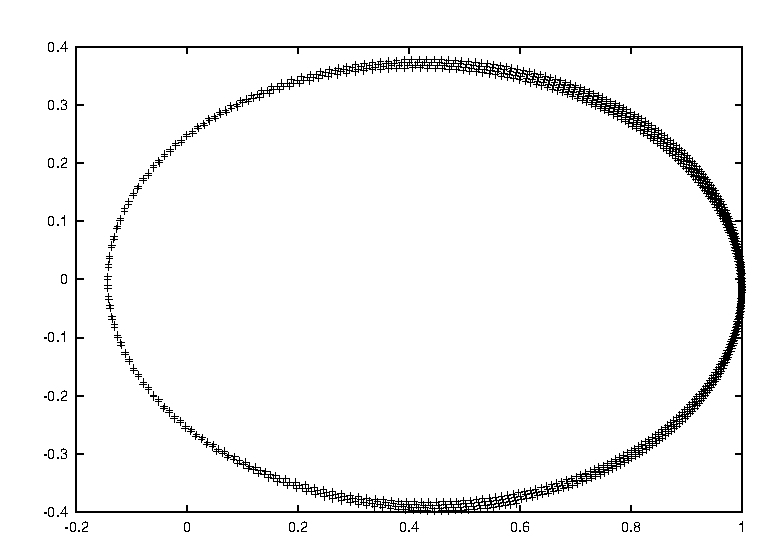
\includegraphics[width=4.5in]{chap4/leapfrog1_0.01.ps}
\caption[Two-body orbit with a leapfrog integrator, time step $dt = 0.01$]
{Relative orbit for the first attempt to integrate a two-body system with a
leapfrog integrator, with time step $dt = 0.01$}
\label{fig:leap1-0.01}
\end{figure}

\begin{figure}[htb]
\centering
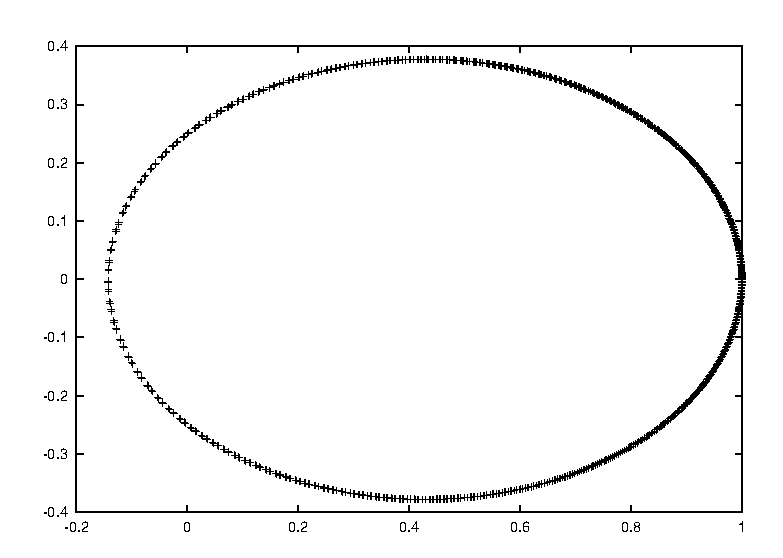
\includegraphics[width=4.5in]{chap4/leapfrog1_0.001.ps}
\caption[Two-body orbit with a leapfrog integrator, time step $dt = 0.001$]
{Relative orbit for the second attempt to integrate a two-body system with a
leapfrog integrator, with time step $dt = 0.001$}
\label{fig:leap1-0.001}
\end{figure}

We can see how the orbit still changes after each revolution, due to
numerical errors, in Fig. \ref{fig:leap1-0.01}.  However, with a time
step of {\st 0.001}, Fig. \ref{fig:leap1-0.001} shows no discernible
errors any more.  Unlike the case with the forward Euler integrator,
the last couple output values for position and velocity differ by only
a few percent at most.  And finally, it is clear that the leapfrog is
indeed second-order: making the time step ten times smaller reduces
the errors by a factor a hundred.  The smaller the time step, the more
accurate this factor of one hundred becomes:

\begin{small}
\begin{verbatim}
|gravity> leapfrog1 > /dev/null
Please provide a value for the time step
0.0001
Initial total energy E_in = -0.875
Final total energy E_out = -0.875
absolute energy error: E_out - E_in = 3.19364e-09
relative energy error: (E_out - E_in) / E_in = -3.64987e-09
|gravity> !!
Please provide a value for the time step
0.00001
Initial total energy E_in = -0.875
Final total energy E_out = -0.875
absolute energy error: E_out - E_in = 3.19509e-11
relative energy error: (E_out - E_in) / E_in = -3.65153e-11
|gravity> !!
Please provide a value for the time step
0.000001
Initial total energy E_in = -0.875
Final total energy E_out = -0.875
absolute energy error: E_out - E_in = 8.60312e-13
relative energy error: (E_out - E_in) / E_in = -9.83214e-13
|gravity> !!
Please provide a value for the time step
0.0000001
Initial total energy E_in = -0.875
Final total energy E_out = -0.875
absolute energy error: E_out - E_in = 1.11888e-12
relative energy error: (E_out - E_in) / E_in = -1.27872e-12
\end{verbatim}
\end{small}

Notice how the scaling first takes this factor 100 to much better than
1\% accuracy, but then flattens off when we begin to approach machine
accuracy for double precision (of order $10^{-15}$).  In the last
case, the cumulative round-off effects are particularly severe.  Not
surprising, given the fact that a time step of {\st dt = 0.000,000,1}
implied a whooping 100,000,000 integration steps, which took a quarter
of an hour to complete.  Whereas the scaling from the first two
outputs would have predicted a final error around {\st 3.20e-15} in
absolute energy and around {\st 3.65e-15} in relative energy, the
actual result shows a turn-up of the error size, paradoxically making
the calculation with one hundred million steps less accurate than the
calculation with ten million steps.

The lesson is to always beware of stretching an algorithm beyond its
natural area of application.  In practice, we will use the leapfrog
when modest accuracy is needed, with errors remaining at a level of,
say, $10^{-4}$ to $10^{-6}$ or so.  If much higher accuracy is needed,
it is better to use a fourth-order scheme, as we will see later on in
this book.
